Given a data path $DP(M_o\cup M_s \cup M_i,I)$, a scheduled D\+FG $G(V_o\cup V_s,E,C)$ and a module library $\Lambda(T,L)$\+:

{\bfseries Module allocation}\+: the {\itshape module allocation} function $\mu :V_o\rightarrow \Pi(M_o)$, determines which module performs a given operation.

Note that a module allocation $\mu(v_i)=m, m\in M_o, v_i\in V_o$ can only be a valid allocation if $m\in \lambda(\tau (v_i))$, i.\+e. the module $m$ is capable of execution of operation type of $v_i$.

{\bfseries Module binding}\+: a {\itshape resource binding} is a mapping $\beta : V_o\rightarrow M_o \times N$, where $\beta(v_o) = (t,r)$ denotes that the operation corresponding to $v_o \in V_o$, with type $\tau(v_o)\in \lambda^{-1}(t)$ (i.\+e. component $t\in L$ can execute the operation represented by vertex $v_o$), is executed on the component $t = \mu(v_o)$ and $r< \sigma(t)$ (i.\+e. the operation is implemented by the {\itshape r-\/th} instance of resource type $t$ and this instance is available into datapath).

A simple case of binding is a dedicated resource. Each operation is bound to one resource, and the resource binding $\beta$ is a one-\/to-\/one function.

A resource binding may associate one instance of a resource type to more than one operation. In this case, that particular resource is shared and binding is a many-\/to-\/one function. A necessary condition for a resource binding to produce a valid circuit implementation is that the operations corresponding to a shared resource do not execute concurrently, i.\+e. they are in mutual exclusion.

When binding constraints are specified, a resource binding must be compatible with them. In particular, a partial binding may be part of the original specification, as described in \hyperlink{src_HLS_binding_constraints_page}{Binding constraints}. This corresponds to specifying a binding for a subset of the operations $U\subseteq V_o$. A resource binding is compatible with a partial binding when its restriction to the operations $U$ is identical to the partial binding itself.\hypertarget{PandA_DOC_intro}{}\section{Introduction}\label{PandA_DOC_intro}
The {\itshape module} {\itshape allocation} is one of subproblems which {\itshape high} {\itshape level} {\itshape synthesis} {\itshape problem} is decomposed in. Here you focus on assignement of modules to all operations into data path.~\newline
~\newline
 First, it\textquotesingle{}s fundamental to give some general definition about module allocation problem and then analyse this and corresponding algorithms implemented.~\newline
~\newline
 \hypertarget{src_HLS_module_binding_page_def_module}{}\section{Module allocation problem definition}\label{src_HLS_module_binding_page_def_module}
Given a data path DP $(M_o\cup M_s\cup M_i,I)$, a scheduled D\+FG $G(V_o\cup V_s,E,C)$ and a module library $\Lambda (T,L)$\+: ~\newline

\begin{DoxyItemize}
\item The {\itshape module} {\itshape allocation} function\+: $ \mu :V_o \rightarrow \Pi (M_o)$ determines which module performs a given operation.
\end{DoxyItemize}

Note that a module allocation $\mu (v_i)=m, m\in M_o, v_i\in V_o$ can only be a valid allocation if $m\in \lambda (\tau (v_i)),$ i.\+e. the module {\itshape m} is capable of execution the operation type of $v_i$.\hypertarget{src_HLS_module_binding_page_comp_graph}{}\subsection{Compatibility graph definition}\label{src_HLS_module_binding_page_comp_graph}
Module allocation problem can be modeled using a module allocation graph. A compatibility graph $G_o(V_o,Y)$ is defined where\+:~\newline
~\newline
 $Y={ \lbrace (v_i,v_j)\mid (\theta (v_i)\cap \theta (v_j)=\emptyset )\vee (m(v_i) \wedge m(v_j)=[0])\wedge \lambda (\tau (v_i)) \cap \lambda (\tau (v_j)) \neq \emptyset \rbrace } $~\newline
~\newline
 An edge $ y\in Y$ is added between two nodes if the two operations they represents can be combined in a single module, i.\+e. the operations do not have to be executed concurrently (they are scheduled into different steps) or are mutually exclusive and there exists a module that can perform both operations.~\newline
 ~\newline
 Despite the fact that the register allocation and module allocation look fairy similar there are some differences. In the register allocation it was quietly assumed that all values could be merged in a register. This may not be the case if registers of different bitwidth are considered. But even in this case the transitivity property remains. If value {\itshape a} and {\itshape b} can be fit into a register and so do {\itshape b} and {\itshape c}, also {\itshape a} and {\itshape c} will fit since there has to be a register of size at least the maximum width of {\itshape a}, {\itshape b} and {\itshape c}. In module allocation this is not necessary the case.  certain restrictions are imposed on the schedule, module allocation can become considerable simpler. If the schedule does not contain operations that are scheduled over multiple cycle steps (multicycling), this will be called a {\itshape simple} schedule. A data flow graph that does not contain conditional branches will be called an {\itshape unconditional} data flow graph.\hypertarget{src_HLS_module_binding_page_library}{}\subsection{Library definitions and properties}\label{src_HLS_module_binding_page_library}
First, some library definitions and proprieties on high level synthesies problem can be given.~\newline
 The data flow graph (graph\+\_\+manager\+::\+D\+FG) describes the input design to a high level synthesis system. A system needs also information on which modules can be used during the synthesis. A collection of these modules are represented by a {\itshape library}. It is common to use a set of modules each of which can only execute a limited set of operations. The {\itshape library} provides a way to describe the relation between the types of operations and the modules.~\newline
~\newline
 The {\itshape library} $ \Lambda (T,L) $ is definited by a set of operation types {\itshape T} and the set of components {\itshape L}. The {\itshape library} {\itshape function} $ \lambda : T \rightarrow \Pi (L) $, determines for each operation type $ t \in T $ by which components it can be performed. So the function $ \lambda ^ {-1}: L \rightarrow \Pi (T) $ describes for each component which types of operations it can execute. The set $ \lambda ^ {-1}(i) $ will be called {\itshape operation} {\itshape type} {\itshape set} of {\itshape l}. Operations whose type belong to the same operation type set can share a module (there is a module that can perform both).~\newline
~\newline
 The {\itshape operation} {\itshape type} {\itshape set} {\itshape function} $ \Omega : L \rightarrow \Pi (O) $, gives for each library component $ l \in L$, which operation types it can execute. The sets $ \Omega (l),l \in L $ will be called the {\itshape operation} {\itshape type} {\itshape sets} of the library $ \lambda (O,L) $.~\newline
~\newline
 A library $ \Lambda (O,L) $ is called a {\itshape ordered} library, if the operation type sets of $ \Lambda (O,L) $ form a partial ordering by the set inclusion relation, where all maximal sets are disjunct, which means that all the maximal sets have not a operation type that can be performed by two different maximal components.~\newline
~\newline
 An ordered set can be depicted conveniently by a Hasse diagram (performed in technology\+\_\+manager\+::check\+\_\+library), in which each element is represented by a point, so placed that if $ X \subset Y $, the point representing X lies below the point representing Y. Lines are drawn to connect sets of {\itshape X} and {\itshape Y} such that {\itshape Y} {\itshape covers} {\itshape X}, i.\+e. $ X \subset Y $ and there is not set {\itshape Z} such that $ X \subset Z \subset Y $; this is implemented by a directed (covering) edge in a look-\/like Hasse diagram. A subset is maximal if it\textquotesingle{}s not covered by any other and so it\textquotesingle{}s maximal if it hasn\textquotesingle{}t any incoming edge.~\newline
~\newline
 A library is called {\itshape complete} if the library is ordered and has only {\itshape one} maximal set.~\newline
~\newline
 A library is called {\itshape ordered} with respect to a D\+FG, if all the operation types in D\+FG are an element of one of the maximal operation type sets. Similary, a library is called {\itshape complete} with respect to a D\+FG, if the maximal operation type set (it\textquotesingle{}s only one) contains all operation types in the D\+FG. In the remainder of this description the terms complete and ordered libreries will always be used with respect to a D\+FG.\hypertarget{src_HLS_module_binding_page_lib_impact}{}\subsection{Impact of libraries on compatibility graphs\+: comparability graphs}\label{src_HLS_module_binding_page_lib_impact}
Now, how a library can impact on module allocation graphs should be analysed.~\newline
~\newline
 First, it could be useful to remember most important properties of {\itshape comparability} {\itshape graphs}.~\newline
 An undirected graph $G(V,E)$ is called a {\itshape comparability} graph if each edge can be assigned a one way direction, in such a way that the resulting oriented graph $G(V,T)$ satisfies the following condition\+:~\newline
~\newline
 $[v_i,v_j]\in T \wedge [v_j,v_k]\in T \Rightarrow [v_i,v_k]\in T$ $\forall v_i,v_j,v_k \in V$~\newline
~\newline
 Comparability graphs are often called {\itshape transitivity} {\itshape orientable} {\itshape graphs}. A relation is called a {\itshape partial} {\itshape ordering} of a set {\itshape A}, when it is reflexive, anti-\/symmetric and transitive. The relation {\itshape T} is a partial ordering defined on a set {\itshape V}, called the {\itshape transitive} {\itshape orientation} of {\itshape G}.~\newline
~\newline
 A module allocation graph derived from an unconditional D\+FG with a simple schedule and a complete library is a comparability graph (and so it\textquotesingle{}s transitive and orientable).~\newline
~\newline
 A module allocation graph derived from and unconditional D\+FG with a simple schedule and an ordered library is a comparability graph.~\newline
 Since the library is ordered the composition will result in a module allocation graph consisting of {\itshape m} disjoint comparability graphs, where {\itshape m} is the number of maximal operation types sets in the library of which elements are present in the data flow graphs. In fact flow\+\_\+allocation can be applied to separated flow network, one for each operation type sets (module\+\_\+binding\+::net\+\_\+flow, passing operation type as a parameter)~\newline
~\newline
 A module allocation graphs derived from a D\+FG with a schedule with property the when operations from a branch are scheduled in the same cycle steps with operations from at most one of its successors branches, and an ordered library, is a comparability graphs.~\newline
 That\textquotesingle{}s why in module\+\_\+binding\+::create\+\_\+graph has been performed a check is D\+FG contains or not only nested conditional operations; in fact, these algorithms can operate also with conditional operations, only if there are not nested.~\newline
~\newline
\hypertarget{src_HLS_module_binding_page_weighted_allocation}{}\section{Weighted module allocation}\label{src_HLS_module_binding_page_weighted_allocation}
We start from a schedule applied before and then operations are been pre-\/allocated by algorithms choosen before. The result is a sequence of scheduled operations, with an initial allocation to operation type sets representing functional units that are in technology library.~\newline
 Module allocation in isolation deals with minimizing the number of operational modules. Now the problem is to improve this module allocation with algorithms exploiting some operation proprieties or considering other aspects of data path allocation. Examples are cost modules or their interconnections. For example, operations can be combined with similar inputs and outputs to reduce the interconnections. Source and destinations of values therefore have to be known. If \hyperlink{src_HLS_registerAllocation_page}{Register allocation} has been performed most inputs and outputs values to the operations are known. So operations can be relocated if results are stored in (or inputs come from) same registers and put in the same functional unit module\+: this has been implemented in module\+\_\+binding\+::weighted\+\_\+allocation (\hyperlink{src_HLS_module_binding_page_threshold}{an algorithm based on progressive thresholds}) and module\+\_\+binding\+::flow\+\_\+allocation (\hyperlink{src_HLS_module_binding_page_flow_net}{flow networks to resolve module allocation problem}) with different algorithms.~\newline
 To model preferences in sharing of operations, weight categories can be assigned to edges in the comparability graph. The edge weight is a measure for the number of common inputs and outputs two operations have (performed in module\+\_\+binding\+::create\+\_\+graph while it\textquotesingle{}s going to create graph). Since the operation nodes are not yet allocated, only the inputs and outputs that have the same operation as origin and destination can be counted. That\textquotesingle{}s been implemented in two different version of module\+\_\+binding\+::get\+\_\+reg\+\_\+op, one for inputs (reading G\+E\+T\+\_\+\+V\+A\+R\+\_\+\+R\+E\+AD list) and one for outputs (reading G\+E\+T\+\_\+\+V\+A\+R\+\_\+\+W\+R\+I\+T\+T\+EN list).\hypertarget{src_HLS_module_binding_page_threshold}{}\subsection{an algorithm based on progressive thresholds}\label{src_HLS_module_binding_page_threshold}
An heuristic algorithm can be used to find the cliques in a weighted graph. The heuristic presented in module\+\_\+binding\+::minimal\+\_\+clique can be extended. Let $ G_{th}(V_{o},Y,W) $ be a graph induced by the edges with weight larger than or equal to the threshold value {\itshape th}. A clique covering is done on this $ G_{th} $. Vertices which form a clique in $ G_{th} $ will be combined in {\itshape G}. Appropriate edges are removed and the weights are update. A new graph is induced with a lower value for the threshold. This process iterates until no new cliques are found and the threshold is low enough to include all remaining edges. ~\newline
 This algorithm has been implemented in module\+\_\+binding\+::clique\+\_\+cover as follow~\newline
 The allocation graph is $ G(V,E)$ (where {\itshape V} is set of clique-\/vertices and {\itshape E} is set of edges) and $ C(T,R)$ is comparability graph (where {\itshape T} is his set of operation-\/vertices and {\itshape R} is his set of edges)\+:~\newline
~\newline
 $\\.find\_maximum\_threshold(C); \\ .\mathbf{foreach}\ op \in T\ \ \mathbf{do} \\ .\ \ \ \ \ v=\lbrace op \rbrace \ \ \textrm{ / / create a vertex-clique with only operation op } \\ .\ \ \ \ \ V=V \cup \lbrace v \rbrace\ \\ .\mathbf{endfor}\\ .\mathbf{foreach}\ ed \in R\ \ \mathbf{do} \\ .\ \ \ \ \ e=\lbrace (s,t)\ \mid s=\lbrace source(ed) \rbrace\ \ \wedge\ \ t=\lbrace target(ed) \rbrace \rbrace\ \ \textrm{ / / populate E } \\ .\ \ \ \ \ E=E \cup \lbrace e \rbrace\ \\ .\mathbf{endfor}\\ .\mathbf{repeat}\\ .\ \ \ \ \ G_{th}=G; \\ .\ \ \ \ \ th=compute\_max\_threshold(G_{th}); \\ .\ \ \ \ \ \mathbf{foreach}\ \ e \in E_{th}\ \ \mathbf{do} \\ .\ \ \ \ \ \ \ \ \ \ \mathbf{if}\ \ weight(e) < th\ \ \mathbf{then} \\ .\ \ \ \ \ \ \ \ \ \ \ \ \ \ \ E_{th} = E_{th} \setminus e \\ .\ \ \ \ \ \ \ \ \ \ \mathbf{endif} \\ .\ \ \ \ \ \mathbf{endfor}\\ .\ \ \ \ \ \ L=compute\_clique\_cover\_on\_G_{th}\ \ \textrm{ / / create a list of clique } \\ .\ \ \ \ \ \mathbf{foreach}\ \ l \in L\ \ \mathbf{do} \\ .\ \ \ \ \ \ \ \ \ \ \ \ n = \emptyset \\ .\ \ \ \ \ \ \ \ \ \ \ \mathbf{foreach}\ \ v \in l\ \ \mathbf{do} \\ .\ \ \ \ \ \ \ \ \ \ \ \ \ \ \ \ \ G=G \setminus \lbrace v \rbrace \\ .\ \ \ \ \ \ \ \ \ \ \ \ \ \ \ \ \ n=n \cup \lbrace v \rbrace \\ .\ \ \ \ \ \ \ \ \ \ \ \mathbf{endfor}\\ .\ \ \ \ \ \ \ \ \ \ \ \ G = G \cup \lbrace n \rbrace \\ .\ \ \ \ \ \ \ \ \ \ \ \ update\_edges\_and\_weights(E) \ \ \textrm{ / / collapse vertices in G graph in a unique clique and update edges } \\ .\ \ \ \ \ \mathbf{endfor}\\ .\mathbf{until}\ \ th>1$~\newline
 See \hyperlink{src_HLS_module_binding_page_Example}{Example} and corresponding \hyperlink{src_HLS_module_binding_page_example_threshold}{resolution with threshold algorithm}

This heuristic will give no guarantee for optimality of the results. In the case of comparability graphs another technique can be employed.\hypertarget{src_HLS_module_binding_page_flow_net}{}\subsection{flow networks to resolve module allocation problem}\label{src_HLS_module_binding_page_flow_net}
Comparability graphs are per definition transitively orientable. If a path $ \langle \ a,b,c\ \rangle $ exists, the edge $ (a,c) $ is guaranteed to exist as well. Each path in the graph will therefore be a clique. So the reminder of this section will describe how to transform the weighted module allocation problem to network flow problem. The transformation to the network flow is a transformation generally valid for comparability graphs. It can therefore be used in the other allocation phases as well.~\newline
~\newline
 Consider the weighted module allocation graph $ G_{o}(V_{o},T,W) $. Furthermore, a source node {\itshape a}, a sink node {\itshape z}, edges from source node to all nodes, edges from all nodes to the sink node and an edge from the sink to the source are added. The edge from the sink to the source is called the {\itshape return} edge, The weight of all these additional edges is zero.~\newline
 Formally, a network $ N_{G}=(V_n,E_n,a,z,C,K) $ corresponding to the module allocation graph is constructed, where\+:~\newline

\begin{DoxyItemize}
\item $ V_n=V_o \cup \lbrace a,z \rbrace $.
\item $ E_n=T \cup \lbrace [a,v],[v,z] \mid v \in V_o \rbrace \cup \lbrace [z,a] \rbrace $.
\item $ w(a,v)=w(v,z)=0\ \ \forall v \in V_o,\ \ \ \ \ \ \ \ \ w(z,a)=0 $.
\end{DoxyItemize}

For each edge $ e \in E_n $ a cost function $ C: E_n \rightarrow \aleph $ is defined, which assigns to each edge a non-\/negative integer. The cost will be equal to the weight of the edges\+: $ C([u,v])=w(u,c) $ for all $ [u,v] \in E_n $.~\newline
 For each edge $ e \in E_n $ a capacity function $ K:E_n \rightarrow \aleph $ is defined, which assigns to each edge a non-\/negative integer. The capacity of all edges is one, except for the return edge which has capacity {\itshape k\+:}  $ K([z,a])=k, \ \ \ \ \ \ \ \ \ \ \ K([u,v])=1 \ \ \ \ \forall [u,v] \in E_n \setminus \lbrace [z,a] \rbrace $.~\newline
~\newline
 A flow in the network $ N_G $ is a function $ f:E_n \rightarrow \aleph ^{+} $, which assigns to each edge a non-\/negative integer, such that for $ e \in E_n,O \leq f(e) \leq K(e) $ and for any node $ u \in V_n $~\newline
 $ \sum _{[u,v]\in E_n} f(u,v) - \sum _{[v,u]\in E_n} f(v,u) \ \ \ \ \ \ \ \ \ \ \ \ \ \ \ \ \ $ balancing equation ~\newline
~\newline
 The amount of flow in the return edge $ [z,a] $ is denoted as $ F=f([z,a]) $. The total cost of the flow is\+: $ k(F)=\Sigma _{e\in E_n} C(e) \cdot f(e) $.~\newline
~\newline
 A flow $ f:E_n \rightarrow \aleph $, in the network $ N_G $ corresponds to a set of cliques $ X_1,...,X_k $ in G\+\_\+o where $ k=F $ .~\newline
~\newline
 The paths $ P_1,...,P_k $ will be edge disjoint (each edge has only capacity=1), but not necessarily go through different nodes (in a node can enter/exit more than one edge). Thus the sets $ X_1,...,X_k $ are not necessarily node disjoint (a node can be in different cliques, so can be allocated into different modules).~\newline
 To enforce node disjoint paths, a node separation technique can be used. In the node separation, all nodes $ v \in V_o $ are duplicated. The duplicate of a node $ v $ is called $ v' $. All edges outgoing from $ v $, obtain the node $ v' $ as their origin. The node $ v $ and its duplicate are connected by an edge with capacity $ K([v,v'])=1 $ (only one unit flow can go through) and a cost $ C([v,v'])=0 $ (no additional solution cost). This node separation results in a network $ N'_G=(V'_n,E'_n,a,z,C',K') $, where\+:~\newline

\begin{DoxyItemize}
\item $ V'_n=V_n \cup V'_o $
\item $ \exists v',v'\in V'_o $ for each vertex $ v \in V_o $
\item $ E'_n=T \cup \lbrace [a,v],[v',z] \mid v \in V_o \rbrace \ \ \cup \ \ \lbrace [z,a] \rbrace \cup \lbrace [v,v']\mid v\in V_o \rbrace $
\item $ T' = \lbrace [v',u]\mid [v,u] \in T\rbrace $
\item $ C'([z,a])=C'([v,v']) = 0 \ \ \ \ \ \forall v \in V_o \ \ \ \ $ (no additional cost for support edges)
\item $ C'([v',u])=C([v,u]) \ \ \ \ \forall [v,v'] \in T' \cup \lbrace [a,v],[v',z]\mid v \in V_o $
\item $ K'([z,a])=k \ \ \ \ \ \ \ \ \ K'([u,v])=1 \ \ \ \ \ \ \forall u \neq z \wedge v \neq a $
\end{DoxyItemize}

Since the capacity of $ K([v,v'])=1 $ at most one unit of flow can go through the edge \mbox{[}v,v\textquotesingle{}\mbox{]}. This leads to the following theorem\+:~\newline
~\newline
 A flow $ f:E'_n \rightarrow \aleph $, in the network $ N'_G $ corresponds to a set of node disjoint cliques $ X_1,...,X_k $ in $ G_o $ where $ k=F $.~\newline
~\newline
 The maximal cost network flow problem finds among all possible flows with amount {\itshape k} the one with maximum cost. This has been implemented in module\+\_\+binding\+::maxcost\+\_\+minflow function, where you can find a way to resolve maxcost flow with a positive cycles elimination. In fact, whenever you can find a positive cycle in the residual network flow, the solution can be incremented over this one and the new solution will be always better. So, if no positive cycles can be found, a better the solution cannot be found and the flow obtained is the maxcost one.~\newline
~\newline
 In this situation, a triple $ (G,s,l) $ is given where $ G=(V,E) $ is a directed graph with {\itshape n} vertices and {\itshape m} edges, $ l:E \rightarrow R $ is a {\itshape lenght} {\itshape function} mapping edges to integer lenghts and $ s \in V $ in the {\itshape root} vertex. The {\itshape lenght} of the path $ \rho = \langle v_0,v_1,...,v_k \rangle $ is the sum of lenghts of its constituent edges (take it negative if the edge is a flow edge due to residual definition graph). So {\itshape positive} {\itshape cycle} is a cycle $ \rho = \langle v_0,v_1,...,v_k,v_o \rangle $ with lenght $ l(\rho )>0 $. Algorithms for P\+CD (positive cycle detection) that use the adjacency-\/list representation of the graph construct a longest-\/path tree $ G_s=(V_s,E_s) $, where $ V_s $ is the set of all vertices reachable from the root {\itshape s}, $ E_s \subseteq E $, {\itshape s} is the root of $ G_s $ and for every vertex $ v \in V_s $ the path from {\itshape s} to {\itshape v} in $ G_s $ is a longest path from {\itshape s} to {\itshape v} in {\itshape G}.~\newline
 The {\itshape labeling} {\itshape method} maintains for every vertex {\itshape v} its {\itshape distance} {\itshape label} $ d(v) $ and parent $ p(v) $. Initially $ d(v)=0 $ and $ p(v)=root $. The method is based on the {\itshape scan} {\itshape operation}. During scanning a vertex {\itshape v}, all edges $ (v,u) $ out-\/going from {\itshape v} are relaxed which means that if $ d(u) < d(v) + l(v,u) $ then $ d(u) $ is set to $ d(v)+l(v,u) $ and $ p(u) $ is set to {\itshape v}. If all vertices have been scanned then {\itshape d} gives the longest path lenghts and $ G_p $ (parent graph induced by edges $ (p(v),v) $) is the longest path tree. So, if there is a cycle, after a finite number of scan operations ( $ \mid V_g \mid $ is upper bound) you can detect it; in fact, starting from a vertex $ v_o $, if the same vertex $ v_o $ is in parent tree, it means that there is a (positive) path from $ v_o $ to $ v_o $, so there is a cycle.~\newline
 Once detected a positive cycle, the flow on positive edges is increased and the flow on negative ones is decremented. So cycle is eliminated and solution cost will be better. If any positive cycle can be detected, there is no way to improve solution and this will be the best one (maximum cost solution). ~\newline
~\newline
 See \hyperlink{src_HLS_module_binding_page_Example}{Example} and corresponding \hyperlink{src_HLS_module_binding_page_example_flow}{resolution with flow network} ~\newline
~\newline
 When the maximal cost network flow is solved for the network $ N'_G $, a solution to the module allocation problem is found, which takes into account the first order effects of interconnection weights. These first order effects describe the result of combining each pair of operations. Taking into account the influence of this combination on the weights with a third operation, would require a dynamic update of the edge weights due to the cumulative nature of the costs. This aspect has not been implemeted yet in this project.~\newline
 \hypertarget{src_HLS_module_binding_page_Example}{}\section{Example}\label{src_HLS_module_binding_page_Example}
For example, having this D\+FG\+:


\begin{DoxyImageNoCaption}
  \mbox{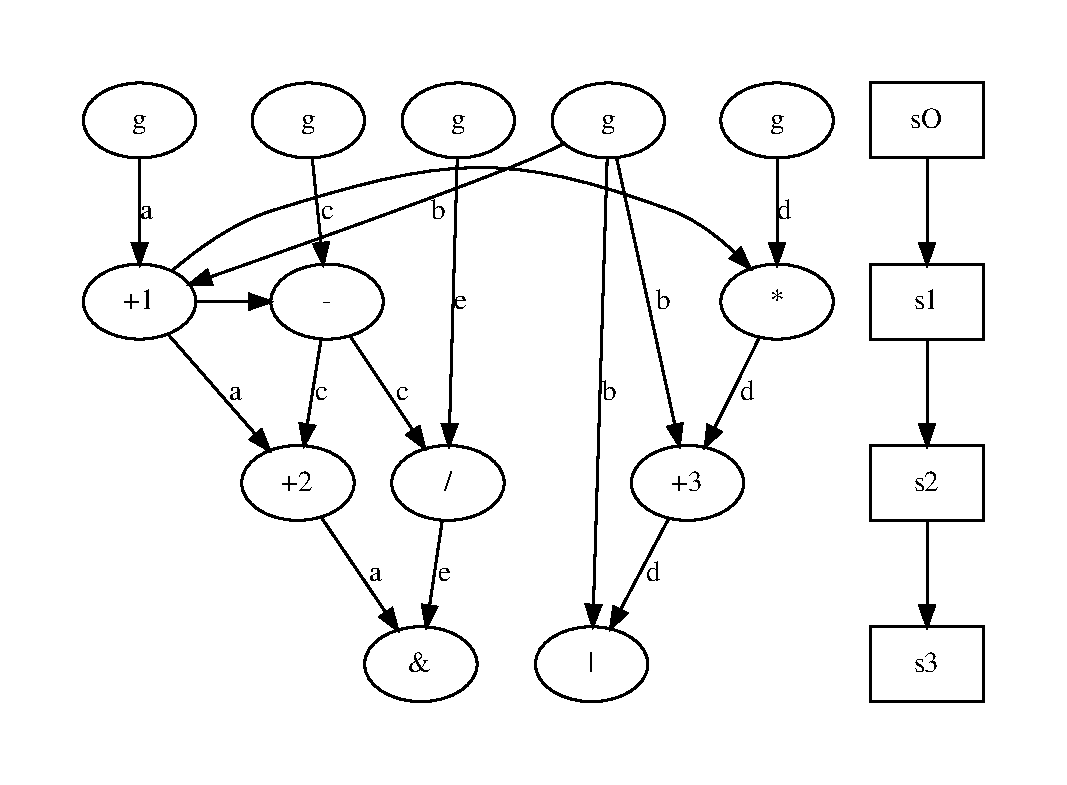
\includegraphics[width=\textwidth,height=\textheight/2,keepaspectratio=true]{dot_inline_dotgraph_12}}
\end{DoxyImageNoCaption}
 where egde label is register name where variable is stored and {\itshape g} are inputs.~\newline
 Assuming a library with two functional unit types, one that can implement $ \lbrace +,-,\&,\mid \rbrace $ and the other that implements $ \lbrace *,/ \rbrace $, comparability graph has to be created, according to definition given above (they are scheduled into different steps or they are in exclusive paths, they can be executed by same functional unit type). 
\begin{DoxyImageNoCaption}
  \mbox{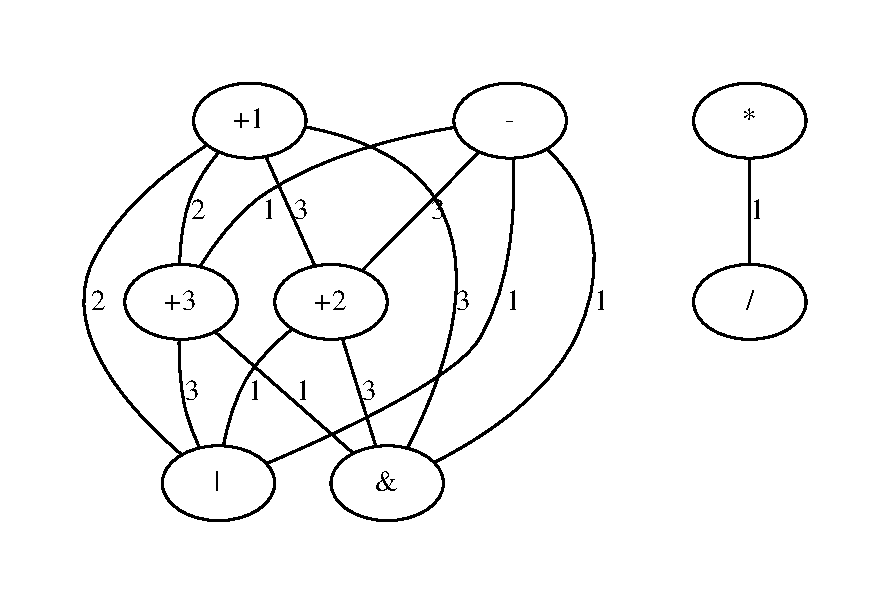
\includegraphics[width=\textwidth,height=\textheight/2,keepaspectratio=true]{dot_inline_dotgraph_13}}
\end{DoxyImageNoCaption}
 \hyperlink{structEdge}{Edge} label is weight value\+: number of commun inputs and outputs. For example, edge $ ('+1','+3') $ has $ w(e)=2 $. In fact, assuming $ w(e)=1 $ as base, that means only one common input or output\+: that is register $ b $ that is a common input\+: both read from this one. \hyperlink{structEdge}{Edge} $ ('+1','+2') $ has a common input (they read both from register $ a $) and a common output (they write both to register $ a $); so it has $ w(e)=3 $. Now, cliques have to be found in this (weighted) graph. It\textquotesingle{}s important to notice that to do this a schedule and an assignement to functional units types have to be provided. These are provided by H\+LS class.\hypertarget{src_HLS_module_binding_page_example_threshold}{}\subsection{resolution with threshold algorithm}\label{src_HLS_module_binding_page_example_threshold}
On the example above, threshold algorithm can be applied as described.~\newline
 First maximum threshold is $ th=3 $ and so graph induced is\+: 
\begin{DoxyImageNoCaption}
  \mbox{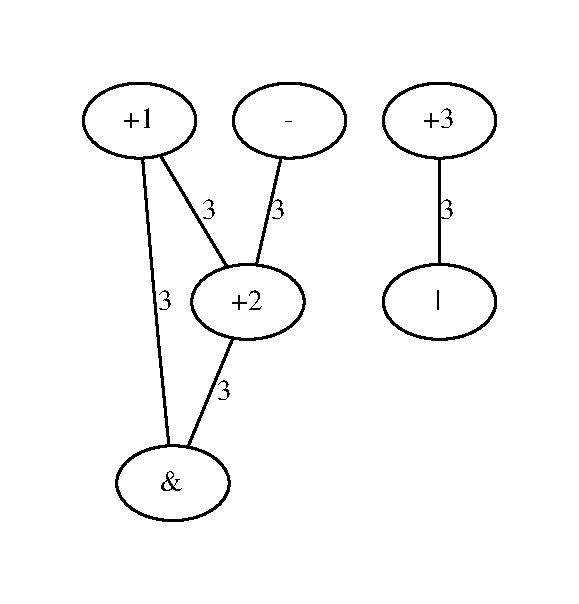
\includegraphics[width=\textwidth,height=\textheight/2,keepaspectratio=true]{dot_inline_dotgraph_14}}
\end{DoxyImageNoCaption}
 where, applying clique covering, three clique can be found\+: $ \lbrace +1,+2,\& \rbrace $, $ \lbrace +3,| \rbrace $ and $ \lbrace - \rbrace $. So the comparability graph modified collapsing nodes and updating egdes (an edge remains if there was an edge beetween the node and each node in the new clique) is\+:~\newline

\begin{DoxyImageNoCaption}
  \mbox{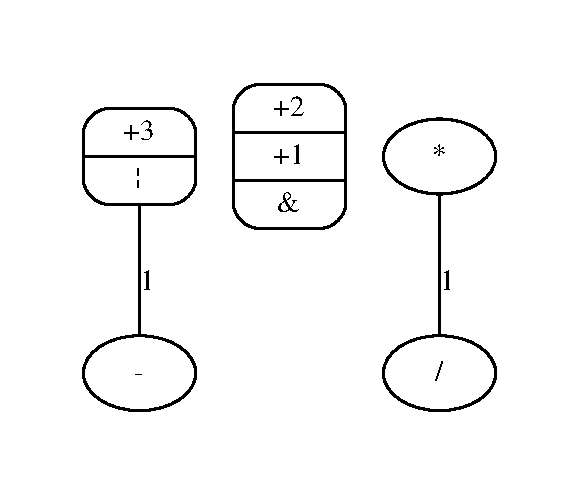
\includegraphics[width=\textwidth,height=\textheight/2,keepaspectratio=true]{dot_inline_dotgraph_15}}
\end{DoxyImageNoCaption}
 Now the choose to compute maximum threshold is shown to be efficent. In fact, there is not any edge $ w(e)=2 $ so the computation is applied with $ th=1 $. The graph induced is the same (no edge is eliminated)\+: 
\begin{DoxyImageNoCaption}
  \mbox{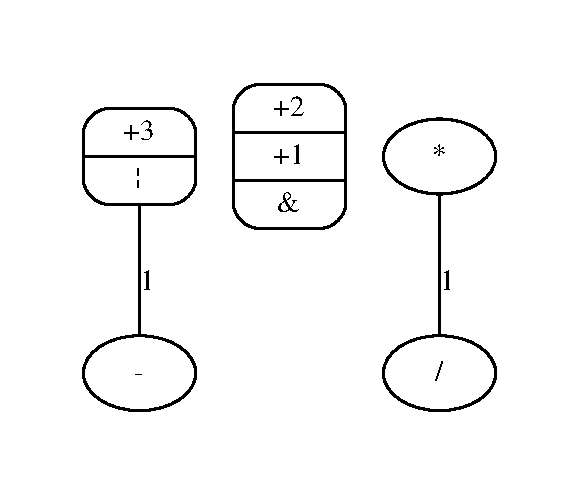
\includegraphics[width=\textwidth,height=\textheight/2,keepaspectratio=true]{dot_inline_dotgraph_16}}
\end{DoxyImageNoCaption}
 and two new clique are found\+: $ \lbrace \lbrace +3, | \rbrace , - \rbrace $ and $ \lbrace *,/ \rbrace $. So, the new (and final) comparability graph is\+: 
\begin{DoxyImageNoCaption}
  \mbox{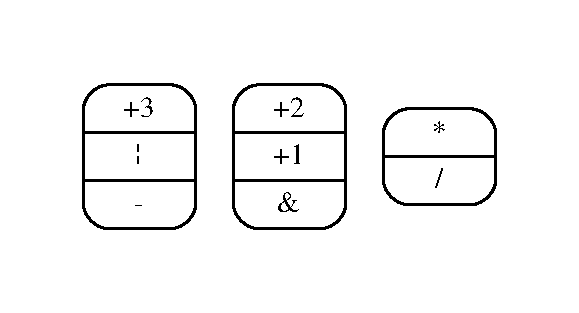
\includegraphics[width=\textwidth,height=\textheight/2,keepaspectratio=true]{dot_inline_dotgraph_17}}
\end{DoxyImageNoCaption}
 No edge is left and so vertices are definitive cliques. Each clique can be assigned to a module. So, operations with weighter edges are prefered to be assigned to same module.\hypertarget{src_HLS_module_binding_page_example_flow}{}\subsection{resolution with flow network}\label{src_HLS_module_binding_page_example_flow}
On example above, there is not any nested conditional operation and so the compatility graph is orientable (it becomes a comparability graph). Thus a flow network for each FU type can be created as well. In according to definition given in subsection \hyperlink{src_HLS_module_binding_page_flow_net}{flow networks to resolve module allocation problem}, the flow network for FU type $ \lbrace +,-,\&,\mid \rbrace $ for resulting is\+:


\begin{DoxyImageNoCaption}
  \mbox{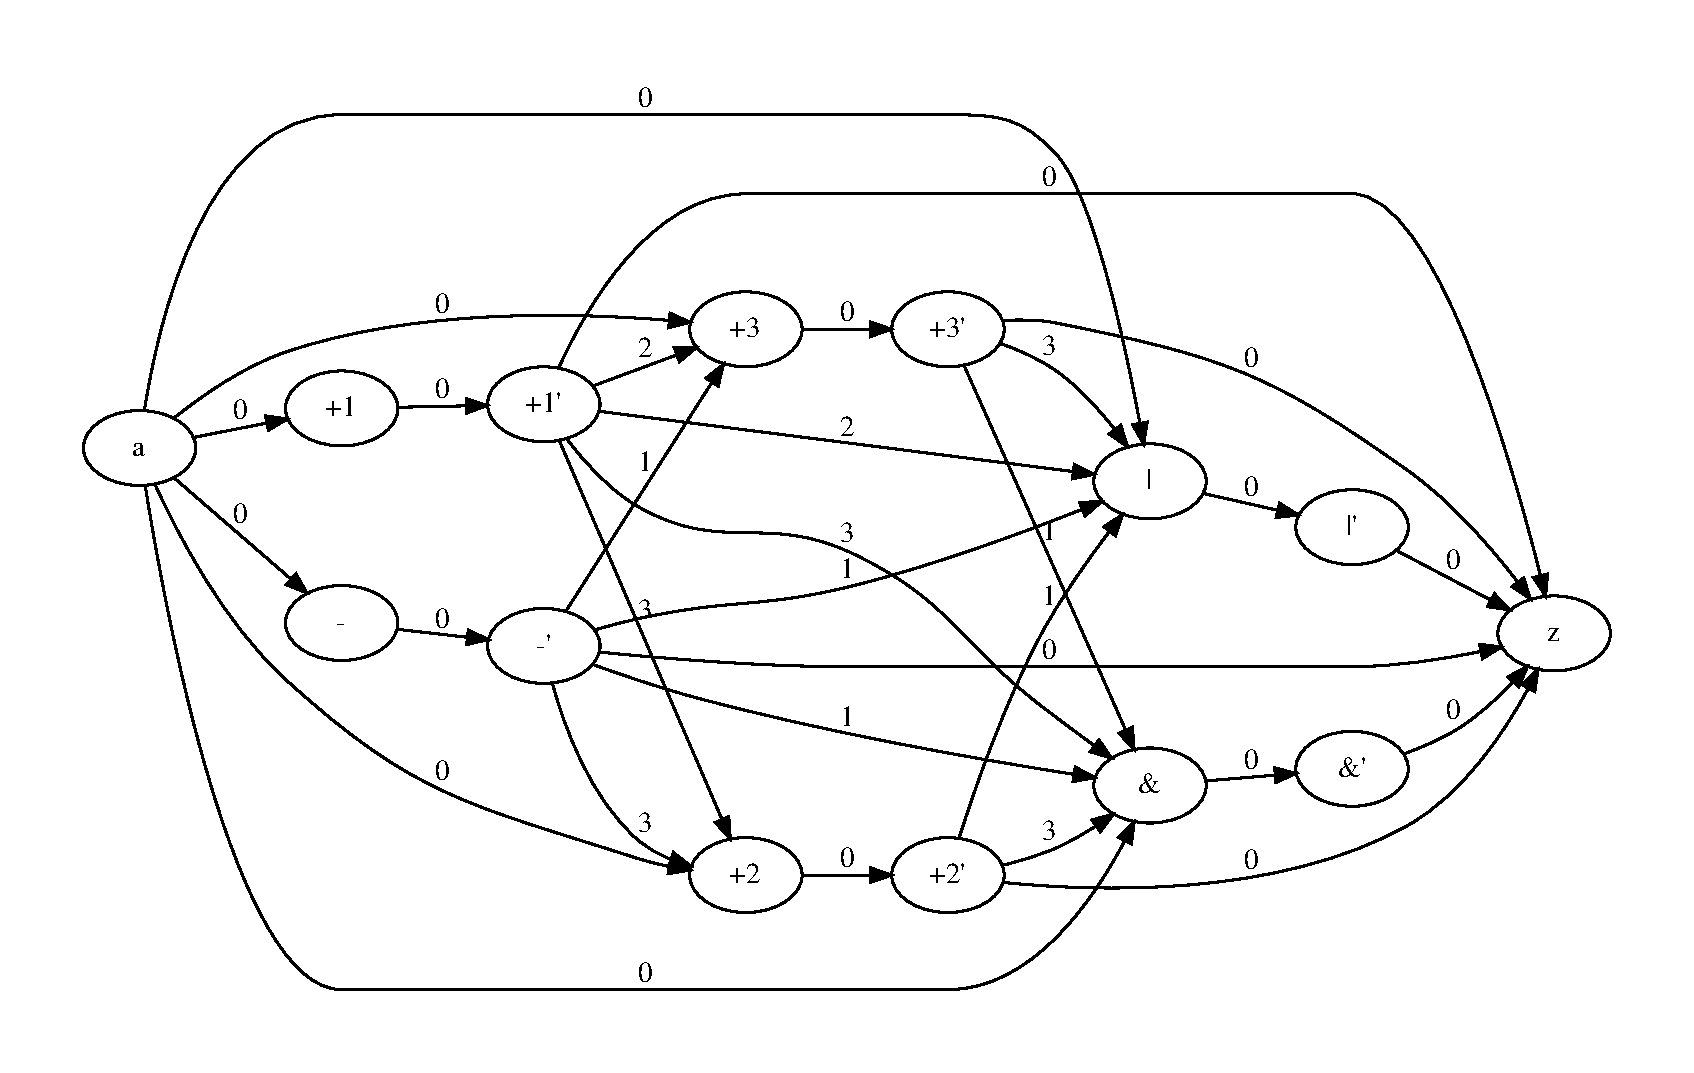
\includegraphics[width=\textwidth,height=\textheight/2,keepaspectratio=true]{dot_inline_dotgraph_18}}
\end{DoxyImageNoCaption}


A dummy initial flow can be applied and corresponding residual graph will be\+:


\begin{DoxyImageNoCaption}
  \mbox{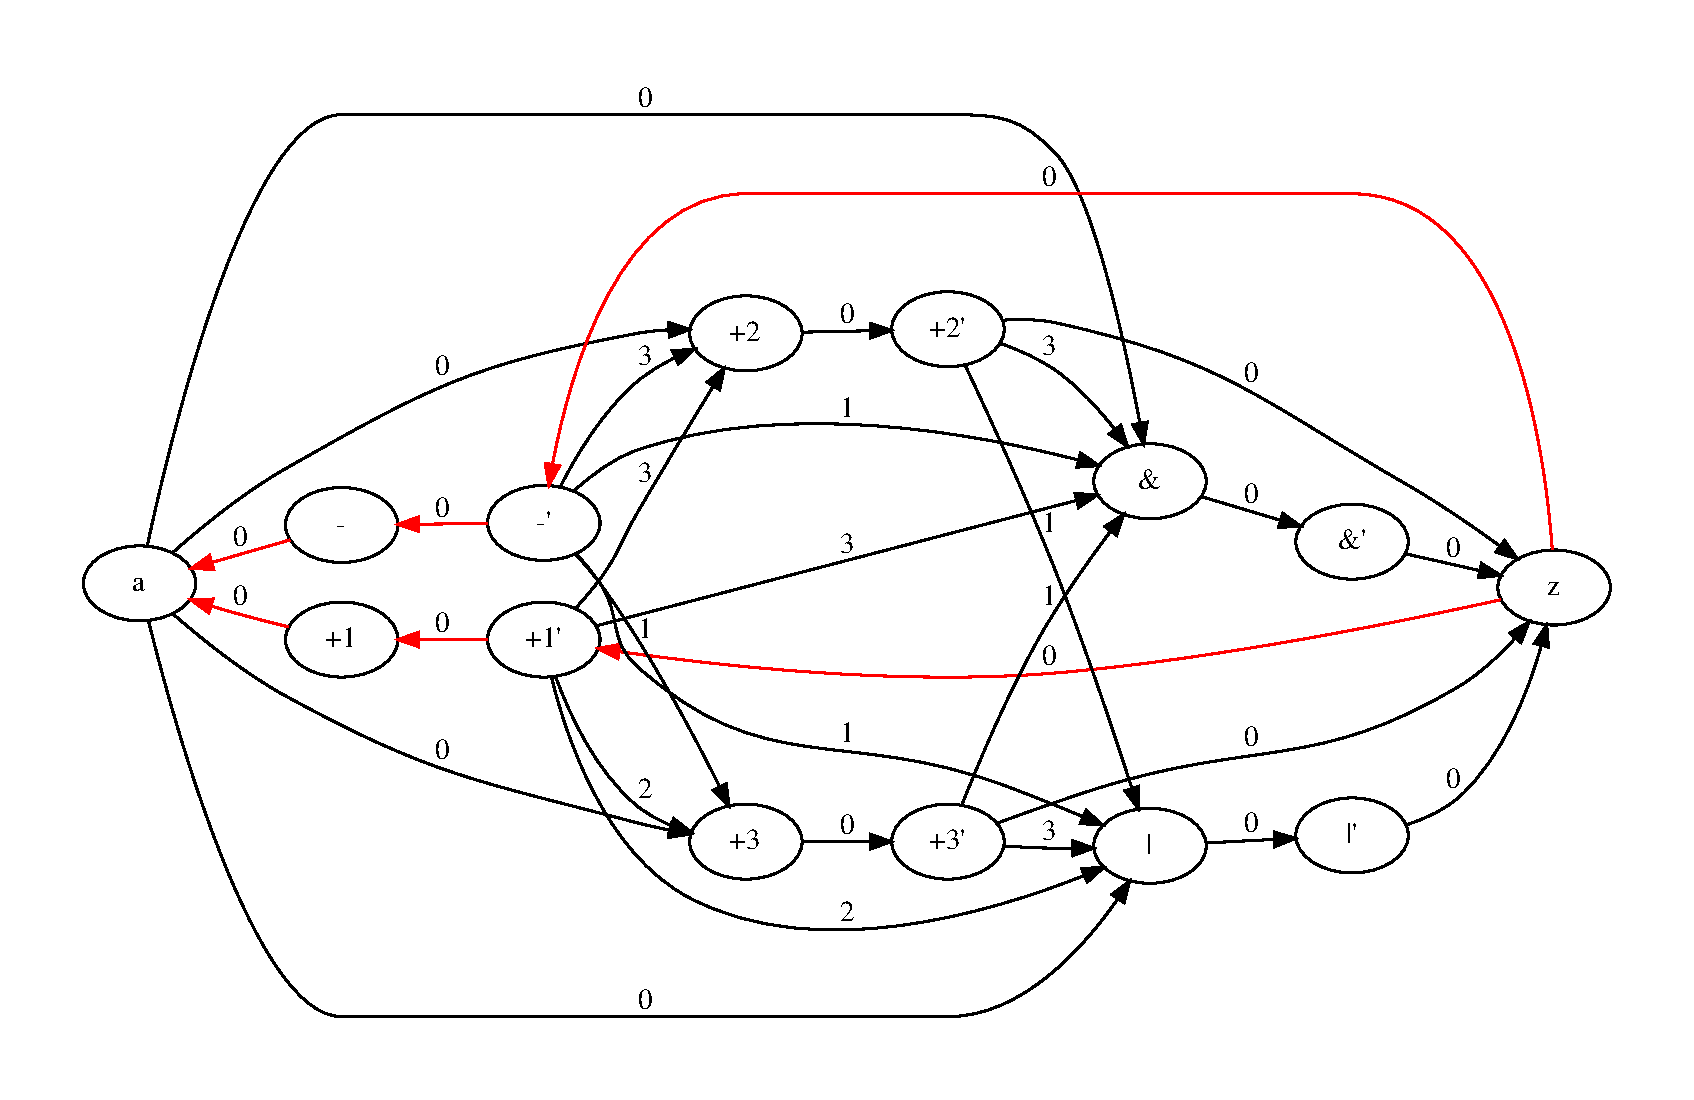
\includegraphics[width=\textwidth,height=\textheight/2,keepaspectratio=true]{dot_inline_dotgraph_19}}
\end{DoxyImageNoCaption}


In this way, it\textquotesingle{}s simple to find a better solution. When a positive cycle has been found (for example $ \rho= <-',+2,+2',z,-'> $ and $ l(\rho )=3) $, the flow can be increased on direct edge and decreased in return edge. Thus solution would be better (from $ C=0 $ to $ C=3 $)\+: 
\begin{DoxyImageNoCaption}
  \mbox{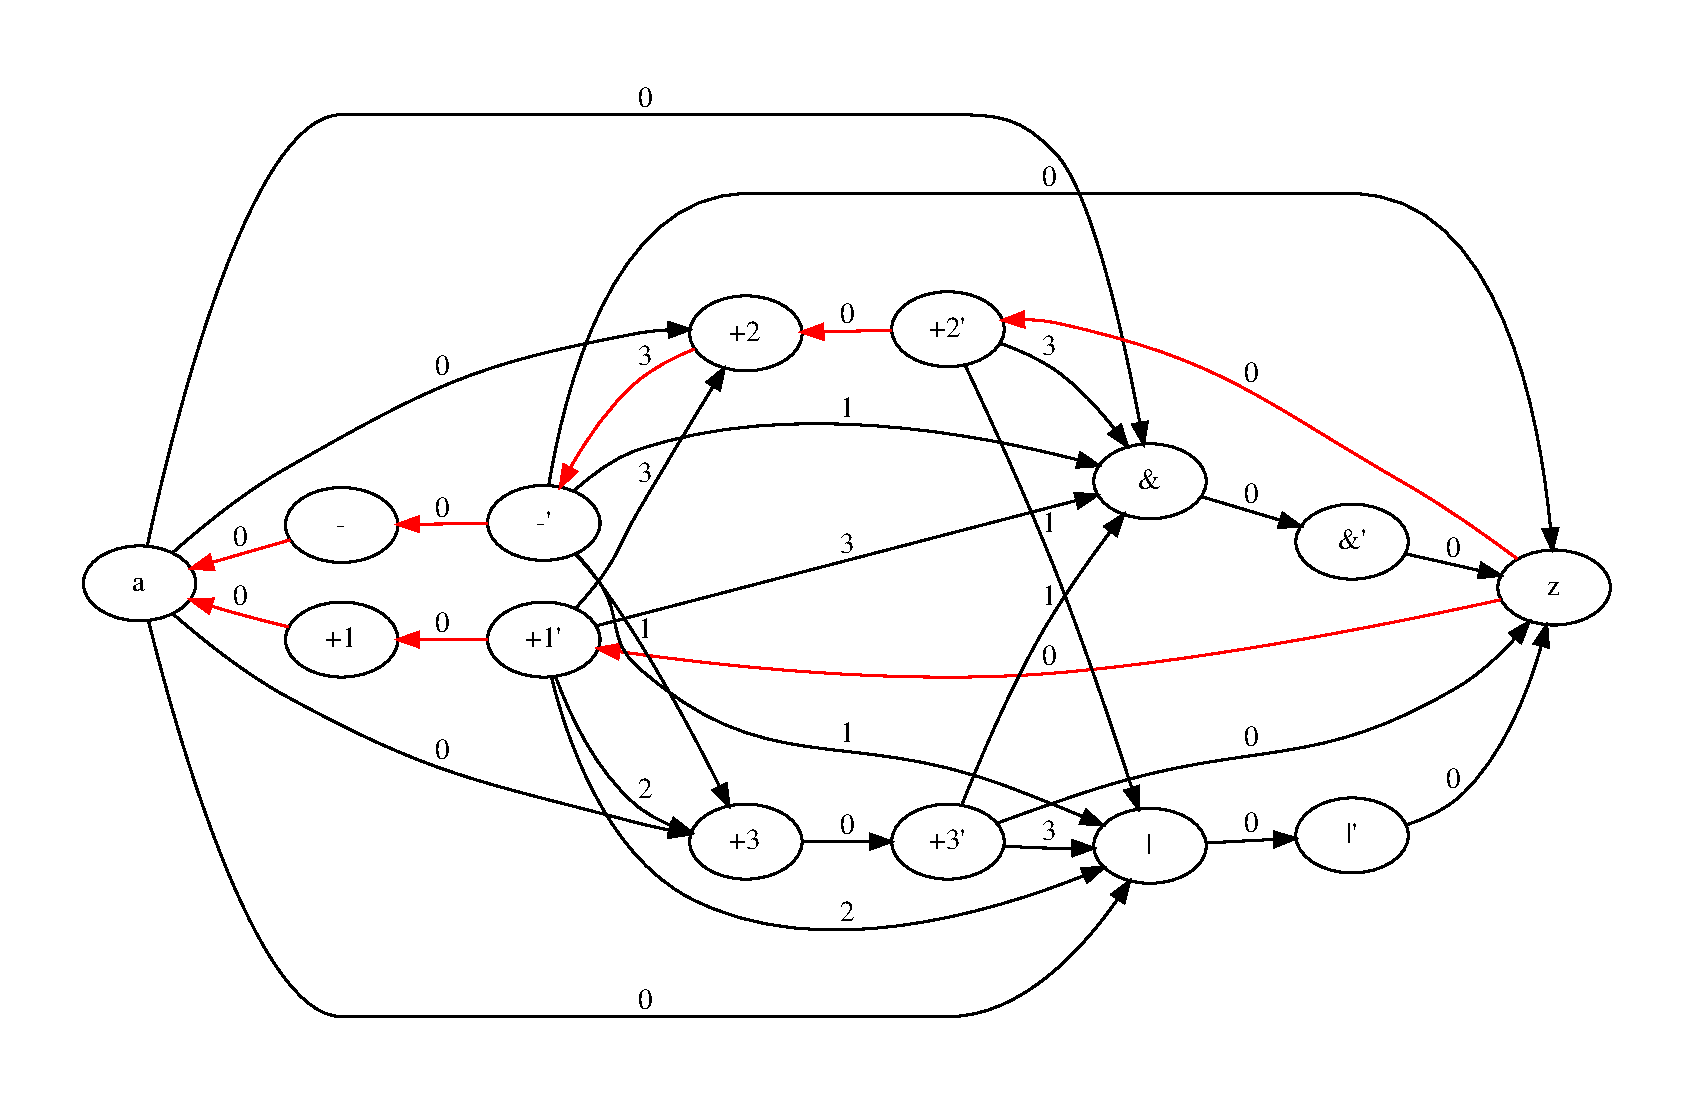
\includegraphics[width=\textwidth,height=\textheight/2,keepaspectratio=true]{dot_inline_dotgraph_20}}
\end{DoxyImageNoCaption}


When no more positive cycles can be found, the solution is optimal for this network and the paths from source to sink will be the max cost partitioning for operation vertices present in this graph. This algorithm have to be applied to all functional units type the library consists in. 